\documentclass[aspectratio=169]{beamer}
\usepackage{ulem}
\usepackage{tikz}
\usepackage{booktabs}
 \usepackage{graphicx,threeparttable,caption}
\usetikzlibrary{shapes,snakes}
\usepackage[beamer,customcolors]{hf-tikz}
\usepackage{nicematrix}
\usepackage{xcolor}
\usepackage{makecell}
\usepackage{array}
\usepackage{csquotes}
\usepackage{csquotes}
\usepackage{minted}
\captionsetup{labelformat=empty,labelsep=none}

\graphicspath{ {./png/} }
\tikzset{hl/.style={
    set fill color=red!80!black!40,
    set border color=red!80!black,
  },
}
\AtBeginSection[]{
  \begin{frame}
  \vfill
  \centering
  \begin{beamercolorbox}[sep=8pt,center,shadow=true,rounded=true]{title}
    \usebeamerfont{title}\insertsectionhead\par%
  \end{beamercolorbox}
  \vfill
  \end{frame}
}
%\usecolortheme[orchid]{structure}
\usetheme[hideothersubsections]{PaloAlto}
\makeatletter
\patchcmd{\csq@bquote@i}{{#6}}{{\emph{#6}}}{}{}
\makeatother
%\usecolortheme{orchid}
%\usefonttheme{professionalfonts}
\newcommand{\soutthick}[1]{%
   \textcolor{red}{
   \renewcommand{\ULthickness}{1pt}%
      \sout{#1}%
   \renewcommand{\ULthickness}{.4pt}% Resetting to ulem default
   }
}
\newcommand{\centered}[1]{\begin{tabular}{l} #1 \end{tabular}}
\setbeamertemplate{section in toc}[square]
\setbeamertemplate{subsection in toc}[square]
\setbeamertemplate{secion in sidebar}[shaded]
\setbeamertemplate{items}[square]
\setbeamercovered{transparent} 

\title[]{Introduction to Computational Social Science}
\subtitle{Introduction}
\author[]{Mikołaj Biesaga\\ \small{\color{blue}{\href{mailto:m.biesaga@uw.edu.pl}{m.biesaga@uw.edu.pl}}}}
\institute{
\includegraphics[width = 4 cm]{uw.png}}
\date{\today}
\begin{document}
\begin{frame}
   \titlepage
\end{frame}

\begin{frame}
    \frametitle{Mikołaj Biesaga}
    \only<1>{
        \framesubtitle{Best Book Ever}
        \begin{center}
            
\includegraphics[width = .3\textwidth]{png/gww.jpg}
        \end{center}
    }
    \only<2>{
        \framesubtitle{Best Books this Year}
        \begin{minipage}{.45\textwidth}
            \begin{center}
                
\includegraphics[width = .7\textwidth]{safekeep.jpg}
            \end{center}
        \end{minipage}
        \begin{minipage}{.45\textwidth}
            \begin{center}
                
\includegraphics[width = .7\textwidth]{brotherlessnight.jpg}
            \end{center}
        \end{minipage}
    }
\end{frame}

\section{Rules of Engagement}

\begin{frame}
    \frametitle{Office Hours, Emails, Presentations, etc.}
    \begin{description}[Google Classroom:]
        \item [Office Hours:] write me an email before coming
        \item [Emails:] the official info will go through emails
        \item [Google Classroom:] materials and presentations will be posted on
        Google Classroom
    \end{description}
    \alert{I will try to answer your inquiries as soon as possible but do not
    count on an immediate response.}
\end{frame}
\begin{frame}
    \frametitle{Emails}
        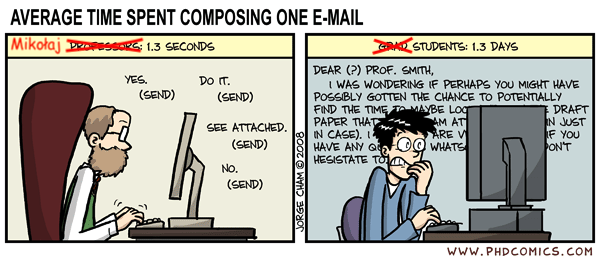
\includegraphics[width = \textwidth]{emails.png}
\end{frame}
\begin{frame}
    \frametitle{Workflow}
    \begin{enumerate}
        \item Introduction to Computational Methods
        \begin{itemize}
            \item Readings at home
            \item Discussion in the classroom
        \end{itemize}
        \item Working with GDELT API
    \end{enumerate}
\end{frame}
\begin{frame}
    \frametitle{Assessment Criteria}
    \only<1>{\begin{itemize}
        \item The final grade will be based on \alert{the final written project} (50 pts), \alert{short tests} (25 pts), and \alert{active participation in the discussions} (25 pts).
        \item Before each class with the discussion (3, 5, 7, 9, and 11), students will submit the title of the chosen scientific article and paragrphaph-long take-home message.
        \item 5 short tests (5 questions each) at the begining of
        the classes 4, 6, 8, 10, and 12.
        \item The research project will require writing a research proposal that uses tools and methods we will cover during the course.
    \end{itemize}
    }
    \only<2>{
        \framesubtitle{Grading Scale}
        \begin{description}
            \item [5\phantom{+} --] => 90 points
            \item [4+ --] 85 - 89 points
            \item [4\phantom{+} --] 75 - 84 points
            \item [3+ --] 70 - 74 points
            \item [3\phantom{+} --] 60 - 69 points
            \item [2\phantom{+} --] =< 59 points
        \end{description}
    }
\end{frame}
\begin{frame}
    \frametitle{Attendance}
    \only<1>{
        \begin{itemize}
            \item You are allowed to miss up to \alert{2 classes in case of a formal excuse}.
            \item Additionally, you are allowed to miss up to \alert{2 classes in the case of a formal excuse}.
            \item An absence does not exempt from submitting the title and summary of the article.
            \item An absence without a formal excuse does not allow to retake
            the short test.
        \end{itemize}
    }
    \only<2>{
        \begin{center}
            
\includegraphics[width = .7\textwidth]{png/pretty_please.jpg}
        \end{center}
    }
\end{frame}

\section{Objectives}

\begin{frame}
    \frametitle{Objective of the course}
    \begin{itemize}
        \item<1> present basic concepts and methods of computational social science
        \item<1> present the advantages, challenges, and limitations of computational methods in social science
        \item<1> teach you how to use some of the discussed methods in practice (sentiment analysis, API)
        
    \end{itemize}
    \only<2>{
        \begin{tikzpicture}[overlay]
            \node[anchor = base, text=red, text width = 13cm, align = center] at ([xshift=-1cm,yshift=-3cm]current page.center){\LARGE This is not a Computer Science Class!};
        \end{tikzpicture}
    }
\end{frame}

\section{CSS}

\begin{frame}
    \frametitle{What is Computational Social Science?}
    \begin{definition}{}
        In the most general sense \emph{Computational Social Science} is a data-driven approach that uses computational methods in studying social phenomena.
    \end{definition}
    \begin{definition}{}
        \emph{Data Science} on the other hand is a broader term than Computational Social Science. It describes the theory and practice of extracting knowledge and insight from data.
    \end{definition}


\end{frame}

\begin{frame}
    \frametitle{Traditional Research Methods}
        \only<+>{
            \begin{itemize}
                \item surveys
                \item observational studies
                \item experiments
                \item case studies
                \item event sampling methodology (diaries)
                \item interviews
                \item meta-analysis
            \end{itemize}}
        \only<+>{
            \resizebox{\textwidth}{!}{
                \begin{tabular}{l | c | c | c | c | c | c }
                Id & Sex & Age & Condition & Variable A & Variable B & Variable C\\
                \hline \hline
                AAA & M & 24 & exp & 55:53 & 3 & apple\\
                AAB & F & 22 & exp & 53:47 & 2 & banana\\
                AAC & F & 28 & con & n/a   & 4 & banana\\
                AAD & M & 21 & con & 54:35 & 3 & banana
                \end{tabular}}
        }
\end{frame}

\begin{frame}
    \frametitle{Computational methods}
    \only<1,3,5,7,9,11>{
        \begin{itemize}
            \item<1> extraction of unstructured data from external digital (i.e. web-based) sources
            \item<3> analysis of textual data (natural language processing -- NLP)
            \item<5> designing experiments
            \item<7> working with big datasets 
            \item<9> network and relational data analysis
            \item<11> computer simulations
        \end{itemize}
    }
    \only<2>{
        \centering
        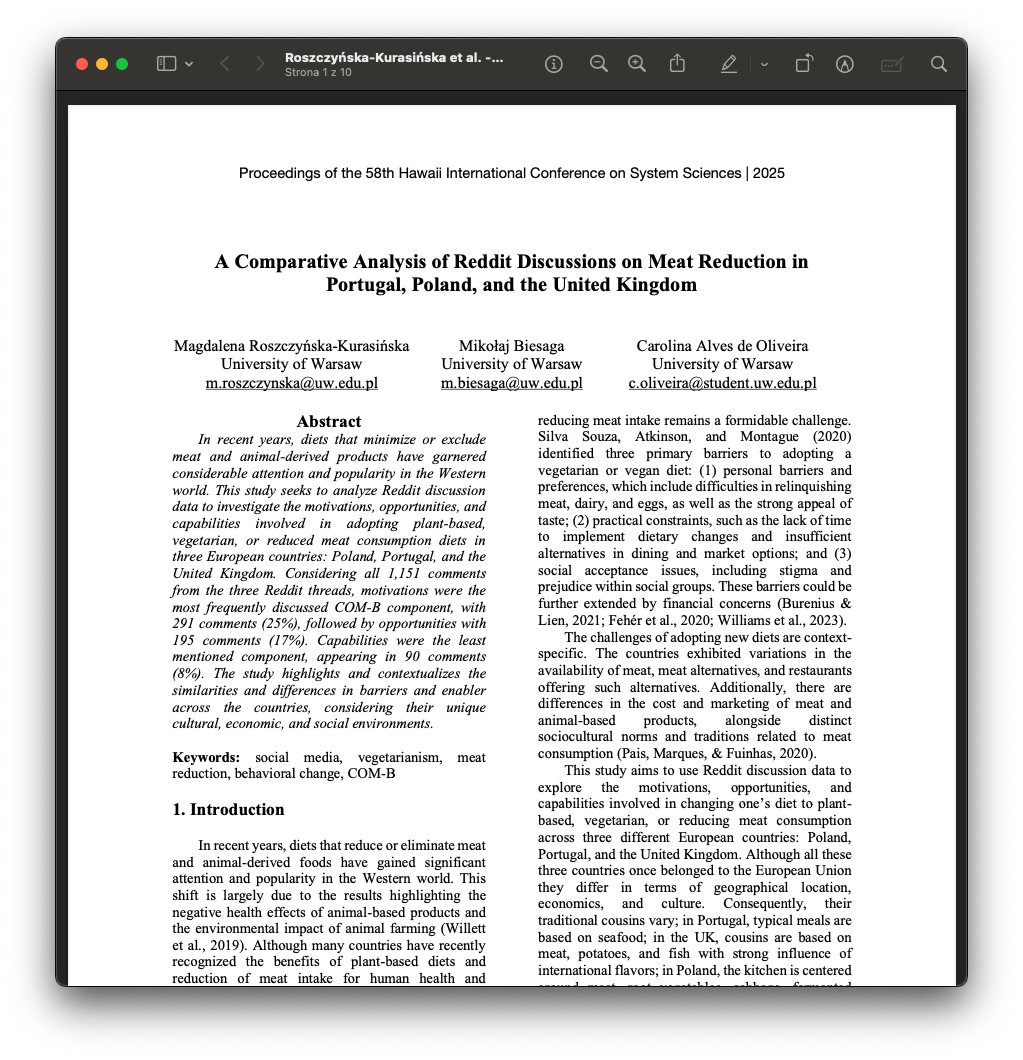
\includegraphics[width = .7\textwidth]{png/carolina.png}
    }
    \only<4>{
        \centering
        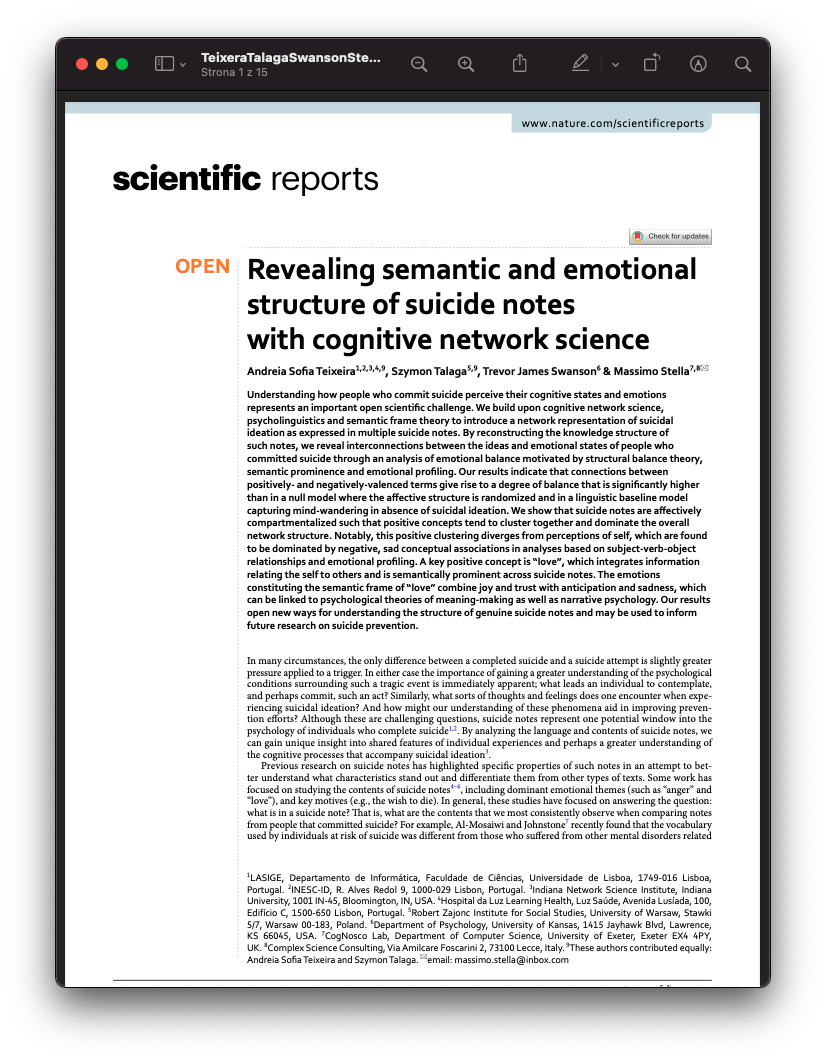
\includegraphics[width = .7\textwidth]{png/nlp.png}
    }
    \only<6>{
        \centering
        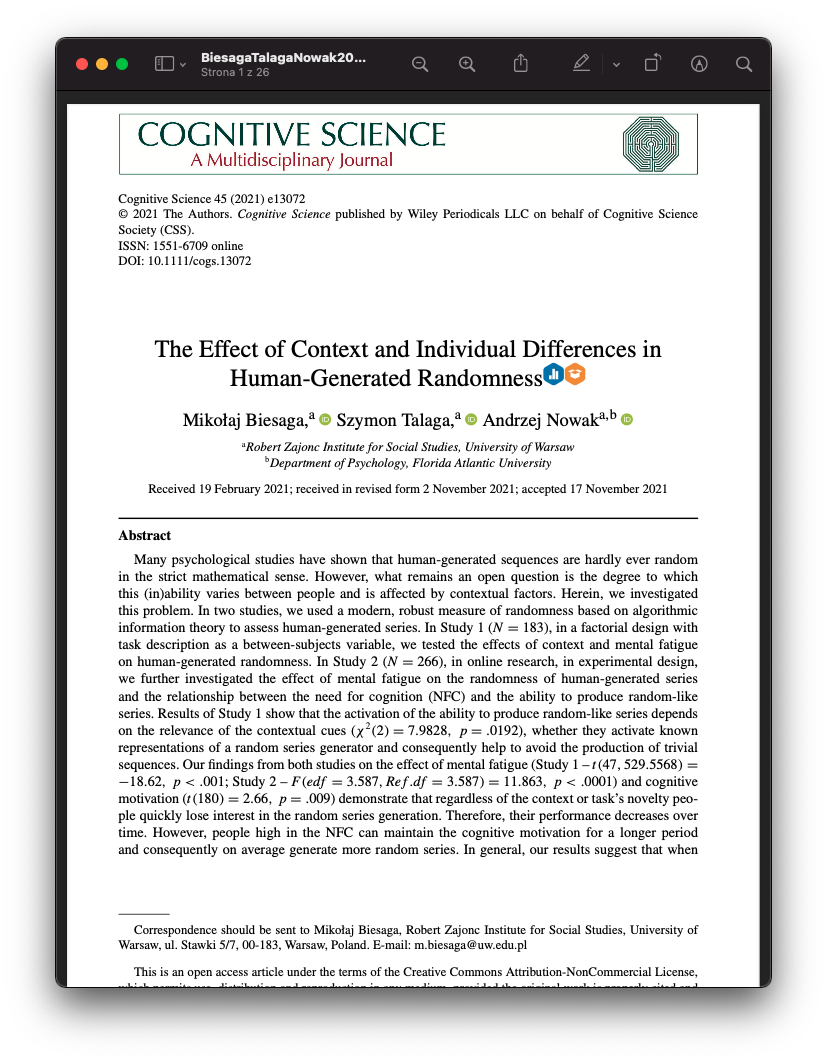
\includegraphics[width = .7\textwidth]{png/designing.png}
    }
    \only<8>{
        \centering
        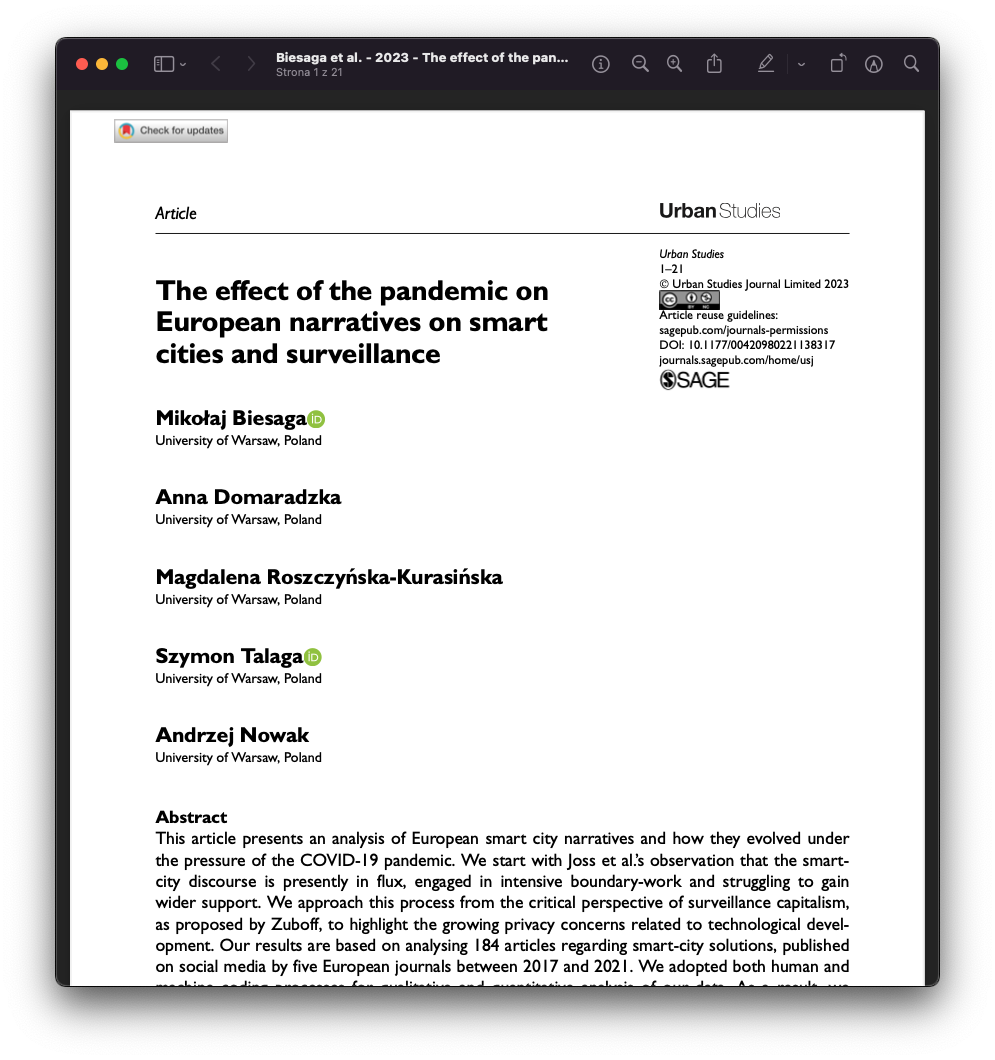
\includegraphics[width = .7\textwidth]{png/big_data.png}
    }
    \only<10>{
        \centering
        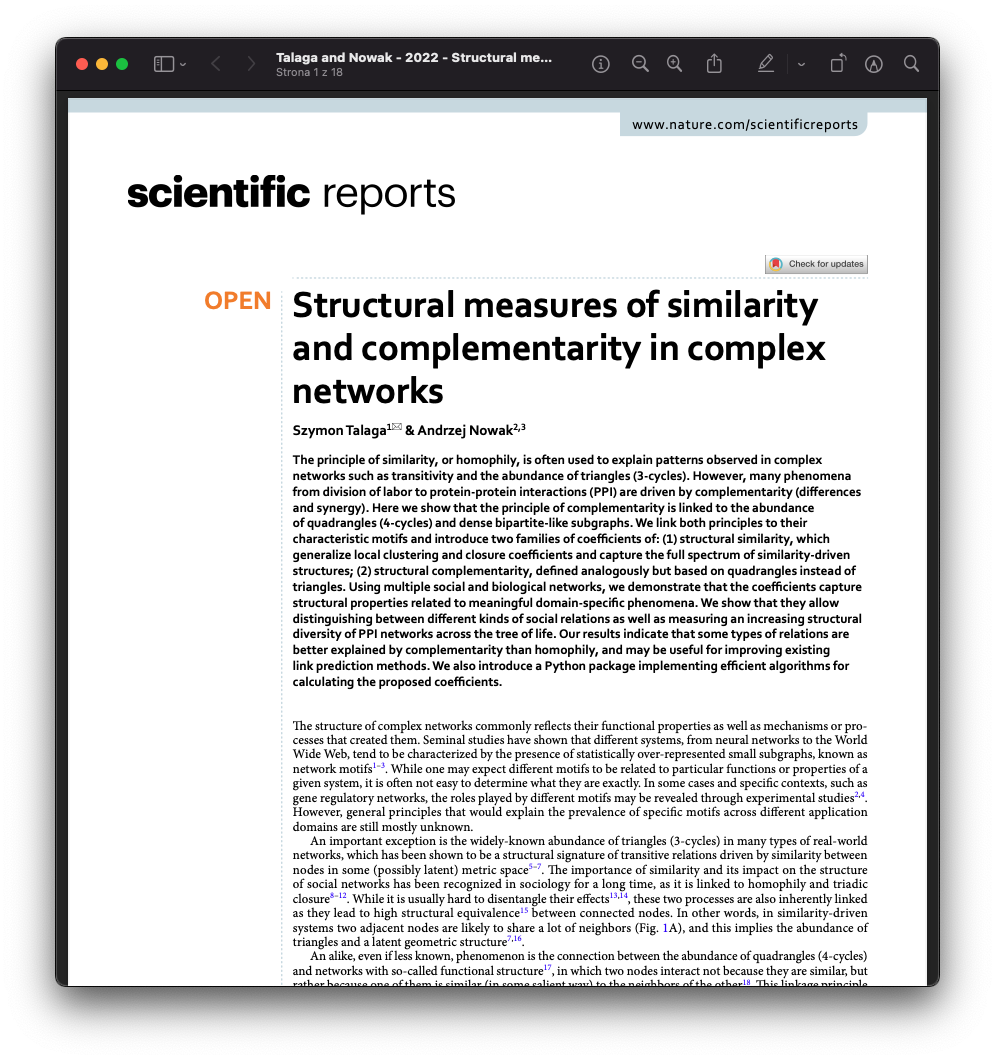
\includegraphics[width = .7\textwidth]{png/networks.png}
    }
    \only<12>{
        \centering
        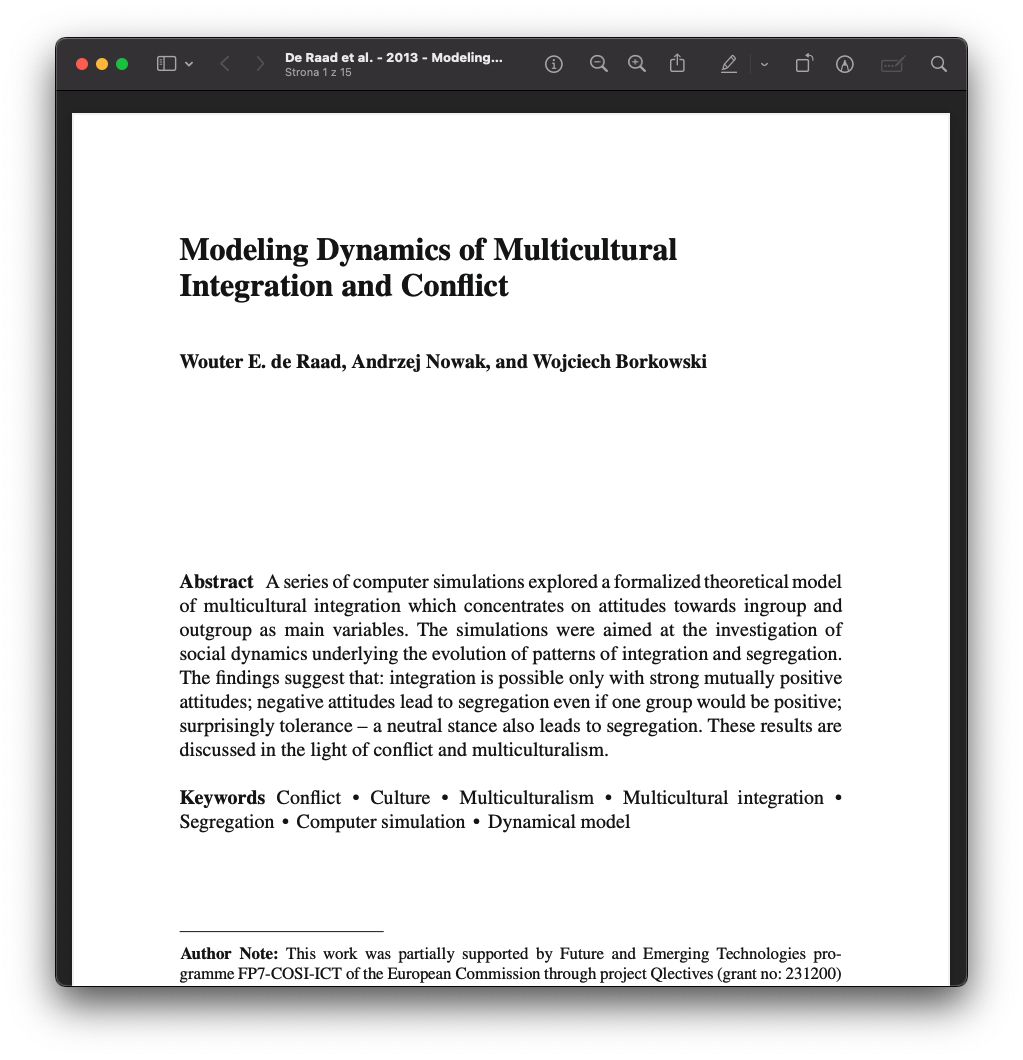
\includegraphics[width = .7\textwidth]{png/wouter.png}
    }

\end{frame}

\section[Data]{Data}

\subsection[Data Sources]{Data Sources}
\begin{frame}
    \setbeamercovered{transparent}
    \frametitle{Data Sources}
    \only<+>{
        \begin{figure}
            
\includegraphics[scale=.35]{png/data_everywhere.png}
        \end{figure}}
    \only<+>{
        \begin{figure}
            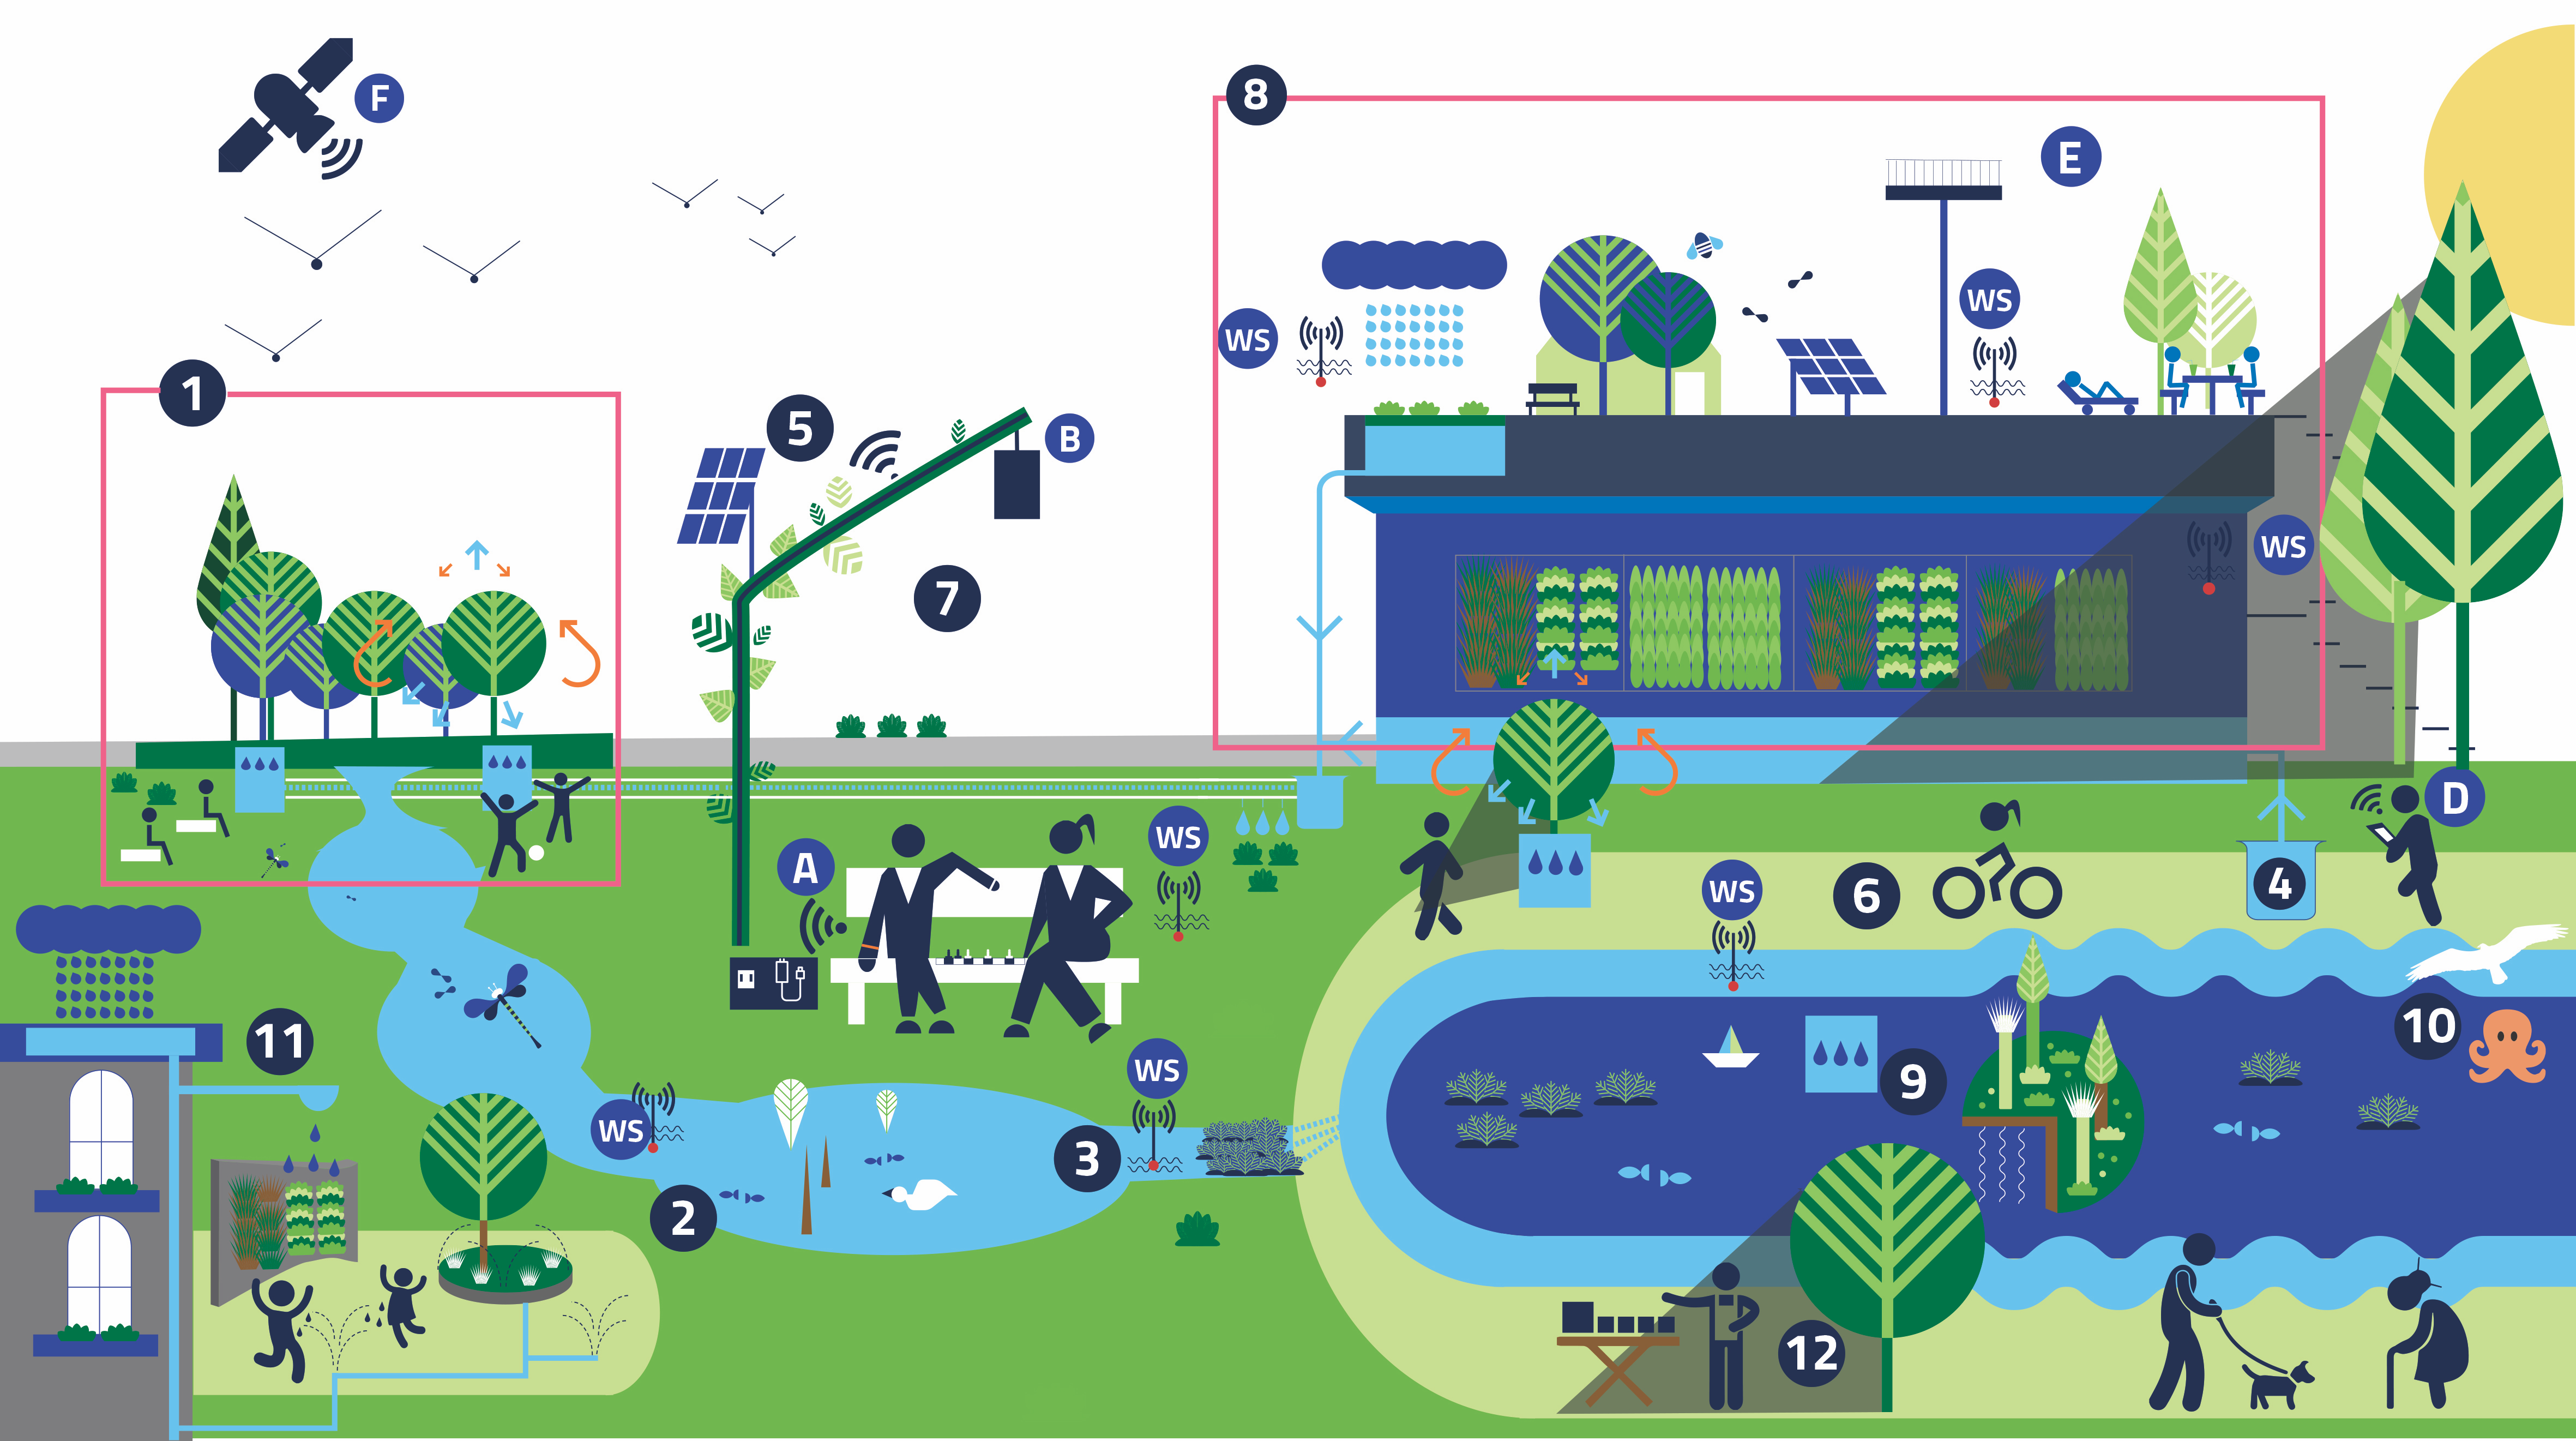
\includegraphics[width = .9\textwidth]{png/mierzenie.png}
        \end{figure}
    }
    \only<+>{
        \begin{figure}
            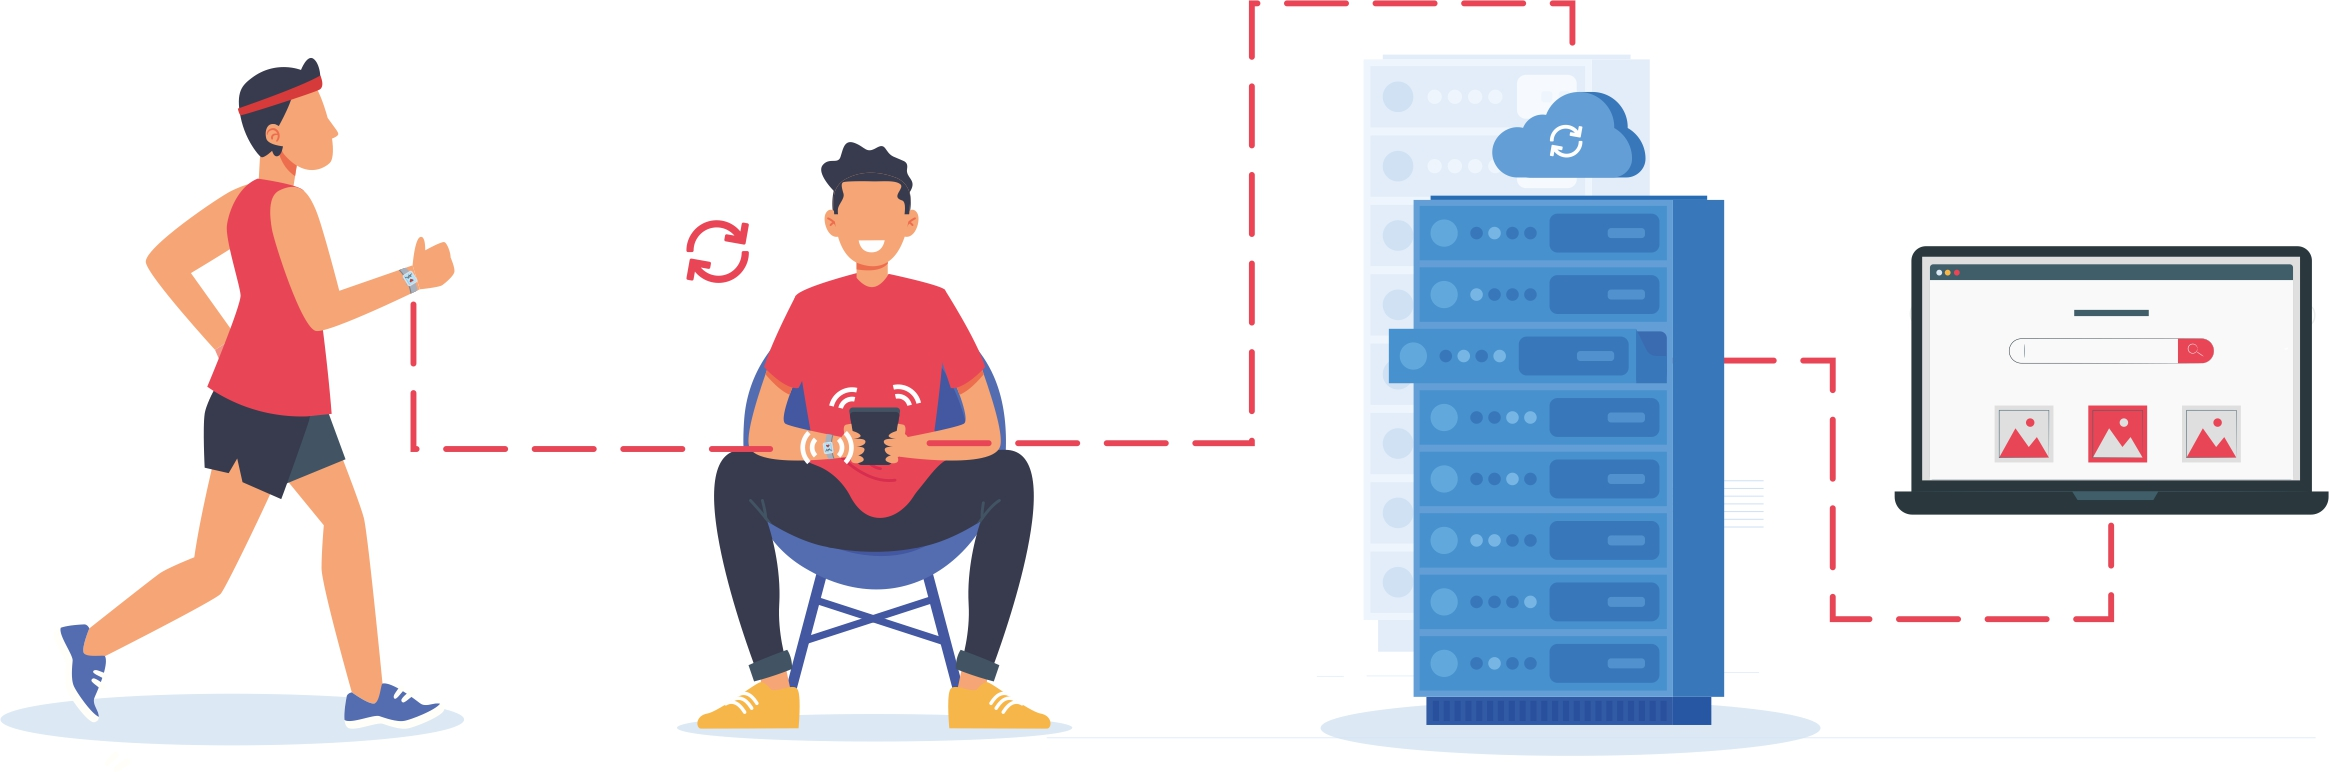
\includegraphics[scale = .5]{png/tracker.jpg}
        \end{figure}
    }
    \only<+>{
        \begin{itemize}
            \item<4> webpages
            \item<4> social media
            \item<4> smart devices
            \item<4> digital behavioral data
            \item<4> mobile phone networks
            \item<4> goverment data
            \item <4>...
        \end{itemize}
        \action<4>{\alert{The fact that you can get the data does not mean you should.}}
    }
\end{frame}


\begin{frame}
    \frametitle{For the next week}
    \begin{itemize}
       \item \textcolor{blue}{\href{https://www.theguardian.com/us-news/2015/dec/11/senator-ted-cruz-president-campaign-facebook-user-data}{Ted Cruz using firm that harvested data on millions of unwitting Facebook users}}
       \item Kosinski, M., Stillwell, D., \& Graepel, T. (2013). Private traits and attributes are predictable from digital records of human behavior. \textit{Proceedings of the National Academy of Sciences}, \textit{110(15)}, 5802–5805. \textcolor{blue}{\href{https://doi.org/10.1073/pnas.1218772110}{https://doi.org/10.1073/pnas.1218772110}}
    \end{itemize}
    
\end{frame}

\end{document}